\section{Sur les déplacements imposés}\label{Ch-DispLag}% et les multiplicateurs de Lagrange}

\medskip
\subsection{Problème considéré}

Nous repartons de l'élément de barre 1D défini au paragraphe~\ref{Sec-barre1D}, et nous rappelons que la matrice de rigidité élémentaire et le vecteur des forces nodales élémentaires sont:
\begin{equation} \MM{K} = \frac{2EA}L \MM*{1 & -1\\ -1& 1} %\end{equation}
\qquad \text{ et } \qquad
\VV{f} = \rho g A \frac{L}4 \VV*{1 \\1} \end{equation}
\medskipvm
L'assemblage de trois éléments, décrit au pagraphe~\ref{Sec-ass}, conduit à:
\begin{equation} \MM{K}=\MM{K_1}+\MM{K_2}+\MM{K_3} \qquad \text{ et } \qquad \VV{F}=\VV{f_1}+\VV{f_2}+\VV{f_3} \end{equation}
\medskipvm
On traitera le cas où les trois éléments ont la même longueurs ($L_1=L_2=L_3=L$) et où seul le nœud 4 est soumis à une force.
%\medskip
%Dans ce cas, on obtient les matrices élémentaires:
%\begin{equation}
%[k_1] = \frac{2EA}{L} \left[ \begin{array}{cccc} 1 & -1 & 0 & 0\\ -1& 1 & 0 & 0\\ 0&0&0&0\\0&0&0&0 \end{array}\right]
%\quad
%[k_2] = \frac{2EA}{L} \left[ \begin{array}{cccc}0&0&0&0\\ 0& 1 & -1 & 0\\ 0 & -1& 1& 0\\0&0&0&0 \end{array}\right]
%\quad
%[k_3] = \frac{2EA}{L} \left[ \begin{array}{cccc}0&0&0&0\\0&0&0&0\\0& 0& 1 & -1\\ 0&0 & -1& 1\end{array}\right]
%\end{equation}
%et les forces nodales:
%\begin{equation}
%\{f_1\} = \{f_2\} = \left\{ \begin{array}{c} 0\\0 \\0\\0 \end{array}\right\}
%\quad
%\{f_3\} = \rho g A \frac{L}4 \left\{ \begin{array}{c} 0\\0\\0 \\1 \end{array}\right\}
%\end{equation}
%
%\medskip
%On s'intéresse à la résolution du système~$[K]\{q\}=\{F\}$ avec les conditions aux limites~$u_1=0$.
%Explicitement, on s'intéresse donc à la résolution du système:
%\medskip
On obtient alors un système de type~$\MM{K}\VV{q}=\VV{F}$ à résoudre, avec la condition aux limites~$u_1=0$, qui s'écrit explicitement dans ce cas:
\begin{equation}
\MM*{1 & -1 & 0 & 0 \\ -1 & 2 & -1 & 0 \\ 0 & -1 & 2 & -1\\ 0&0&-1&1}
\VV*{u_1\\u_2\\u_3\\u_4}
=
\VV*{0\\0\\0\\F'}
\end{equation}
(avec~$F'=\rho g L^2/(8E)$).

\medskip
\subsection{Retour sur la résolution de systèmes linéaires}

Soit à résoudre un système linéaire de type:
\begin{equation}\label{Eq-lin} \MM{A}\VV{x}=\VV{b} \end{equation}
Ce système peut être réécrit par blocs sous la forme:
\begin{equation} 
\MM*{A_{11} & A_{12}\\ A_{21} & A_{22}}
\VV*{x_1 \\ x_2} =
\VV*{b_1\\ b_2}
\end{equation}
\medskipvm
Si~$A_{11}$ est inversible, alors on peut écrire la première ligne:
\begin{equation}
x_1 = A_{11}^{-1}\left( b_1-A_{12}x_2 \right)
\end{equation}
ce qui donne, dans la deuxième ligne:
\begin{equation}
A_{22} - A_{21}A_{11}^{-1}A_{12}x_2 = b_2 - A_{21}A_{11}^{-1}b_1
\quad \text{ que l'on note: }
S x_2=c
\end{equation}
\textcolorblue{La matrice~$S$ est appelée complément de Schur}\index{complément de Schur}\index[aut]{Schur (Issai), 1875-1941, Russe} (présenté au paragraphe~\ref{Sec-Schur}), ou matrice condensée sur les degrés de liberté~$x_2$. Ce calcul est également identique à celui présenté à propos de la condensation statique au paragraphe~\ref{Sec-condens}. Dans ce cas, la matrice~$S$ est la matrice de rigidité du super-élément considéré.

\medskip
Le système initial (\ref{Eq-lin}) est équivalent à:
\begin{equation}\label{Eq-Sch1}
\MM*{A_{11} & A_{12}\\ \mO & S}
\VV*{x_1\\ x_2} =
\VV*{b_1\\ c}
\end{equation}
qui peut être réécrit:
\begin{equation}
\MM*{I & \mO{} \\ A_{21}A_{11}^{-1} & I}
\MM*{A_{11} & A_{12}\\ \mO{} & S}
\VV*{x_1\\ x_2} =
\MM*{I & \mO{} \\ A_{21}A_{11}^{-1} & I}
\VV*{b_1\\ c}
\end{equation}

\medskip
\subsection{Complément de Schur et déplacements imposés}\index{complément de Schur}\index[aut]{Schur (Issai), 1875-1941, Russe}

Nous cherchons toujours à résoudre notre système:
\begin{equation}\MM{K}\VV{q}=\VV{F}\end{equation}

\medskip
Considérons la matrice~$\MM{D}$, \textcolorblue{matrice booléenne}, permettant d'extraire de l'ensemble des inconnues nodales~$\VV{q}$ le sous-ensemble~$\VV{q_2}=\MM{D}\VV{q}$ sur lesquels portent les conditions de déplacements imposés~$\VV{q_d}$ \textcolorred{(ici on traite le cas général, i.e. les déplacements imposés peuvent être nuls ou non)}. La matrice \textcolorblue{$\MM{D}$ n'est pas rectangulaire}: si on souhaite imposer~$d$ déplacements parmi les~$n$ degrés de liberté du système, alors~$\MM{D}$ est de dimension~$d\times n$, et donc~$\VV{q_2}$ est bien un vecteur à~$d$ composantes, comme~$\VV{u_d}$.

\medskip
Le système~$\MM{K}\VV{q}=\VV{F}$ peut alors s'écrire, par blocs, en utilisant le complément de Schur (\ref{Eq-Sch1}) sous une forme triangulaire d'où l'on tire le sous-système correspondant aux déplacements non imposés:
\begin{equation}
\MM{K_{11}}\VV{q_1} = \VV{f_1} - \MM{K_{12}}\VV{u_d}
\end{equation}
\medskipvm
Ce système est \textcolorblue{réduit}, i.e. possède moins d'inconnues que le problème initial, mais il est nécessaire de modifier le chargement extérieur.

Son inconvénient est qu'il est nécessaire d'effectuer un \textcolorred{tri explicite} au sein des degrés de liberté, ce qui a pour conséquence de «remplir» le terme~$\MM{K_{12}}$, et par suite peut générer un surcoût de calcul lorsque le nombre de degrés de liberté bloqués est grand.

C'est ainsi que procède le code \abaqus pour imposer les déplacements.

\medskip
\subsection{Multiplicateurs de Lagrange et déplacements imposés}\index{multiplicateurs de Lagrange}\index[aut]{Lagrange (Joseph Louis, comte de -), 1736-1813, Italien}\label{Sec-cast}

Une autre technique, pour imposer des déplacements, consiste à utiliser les multiplicateurs de Lagrange:\index{multiplicateurs de Lagrange}\index[aut]{Lagrange (Joseph Louis, comte de -), 1736-1813, Italien} les contraintes sont relaxées, puis réintroduites via des multiplicateurs de Lagrange.

Dans ce cas, il n'est plus nécessaire de séparer explicitement les degrés de liberté, mais \textcolorred{la taille du problème augmente} puisqu'il faut lui adjoindre les multiplicateurs.

Le système à résoudre s'écrit très simplement:
\begin{equation}\label{Eq-Lag1}
\MM*{\MM{K} & -\MM{D}^T\\ -\MM{D} & \mO{}}
\VV*{q\\ \lambda} =
\MM*{A}
\VV*{q\\ \lambda} =
\VV*{F\\ -u_d}
\end{equation}
Il est intéressant de remarquer que la première ligne montre que \textcolorblue{les multiplicateurs de Lagrange sont bien les réactions aux appuis}.\index{multiplicateurs de Lagrange}\index[aut]{Lagrange (Joseph Louis, comte de -), 1736-1813, Italien}

Par contre, la matrice du système (\ref{Eq-Lag1}), $\MM{A}$, si elle reste bien symétrique, \textcolorred{n'est plus définie positive}. Elle possède des valeurs propres négatives.
\medskipvm
Toutefois, on dispose du résultat suivant:

\begin{theoreme}
si~$\MM{K}$ est symétrique définie positive, alors:
\begin{equation}
\MM{A} \text{ inversible } \Longleftrightarrow \MM{D} \text{ injective } \Longleftrightarrow \ker \MM{D} = \emptyset
\end{equation}
\end{theoreme}
ce qui correspond aux cas où toutes les liaisons sont indépendantes.

\bigskipvm
Afin de ne pas détruire la structure bande de~$\MM{K}$ (ce que ferait une factorisation de Gauß),\index[aut]{Gauß (Johann Carl Friedrich), 1777-1855, Allemand} et d'éviter des pivotages (que ferait une factorisation de Crout, i.e.~$\MM{L}\MM{D}\MMT{L}$), on peut développer une autre technique, dite \textcolorblue{technique de double multiplicateur}, qui est celle employée dans \castem:\index{multiplicateurs de Lagrange}\index[aut]{Lagrange (Joseph Louis, comte de -), 1736-1813, Italien}
\begin{equation}
\left\{\begin{aligned}
&\MM{K}\VV{q} = \VV{F} - \MMT{D}\left(\VV{\lambda_1} - \VV{\lambda_2}\right) \\
&\VV{\lambda_1} = \VV{\lambda_2} \\ 
&\MM{D}\VV{q} = \VV{u_d}
\end{aligned}\right.
\end{equation}
\textcolorred{L'inconvénient reste l'augmentation de la taille du système lorsque l'on a de nombreux blocages.}

\medskip
\subsection{Actions extérieures et déplacements imposés}

L'interprétation physique des multiplicateurs de Lagrange conduit naturellement à une autre méthode: il est possible de considérer un déplacement imposé comme une action extérieure, par exemple comme la réaction d'un ressort ayant une raideur~$k$ très grande et un déplacement imposé à sa base.

\medskip
On se retrouve alors avec un système du type:
\begin{equation}
\left(\MM{K} + \MMT{D}k\MM{D}\right) \VV{q} = \VV{F} + \MMT{D}k\MM{D}\VV{u_d}
\end{equation}
dans lequel on n'a fait qu'ajouter des termes à la matrice de rigidité sur les degrés de liberté correspondant à ces déplacements et au vecteur des forces généralisées sur les efforts duaux.

\medskip
\textcolorred{Le problème réside dans le choix de la valeur de~$k$}: trop petite, la condition est mal imposée; trop grande, le système devient très mal conditionné, voire numériquement singulier.

\medskip
\subsection{Retour sur notre exemple}

Nous devons toujours résoudre:
\begin{equation}
\MM*{1 & -1 & 0 & 0 \\ -1 & 2 & -1 & 0 \\ 0 & -1 & 2 & -1\\ 0&0&-1&1}
\VV*{u_1\\u_2\\u_3\\u_4}
=
\VV*{0\\0\\0\\F'}
\end{equation}
avec la condition aux limites~$u_1=0$.
\medskipvm
Tout d'abord, on pourra essayer de résoudre sans introduire de conditions aux limites afin de voir que le système est alors singulier. On obtient~$u_1=u_2=u_3=u_4$ et~$F'=0$.
\medskipvm
La méthode la plus rudimentaire consiste à prendre en compte directement et explicitement la condition aux limites. On supprime donc du système matriciel la ligne et la colonne correspondant à~$u_1$, et on résout:
\begin{equation}\label{Eq-Base}
u_1=0 \text{ et }
\MM*{2 & -1 & 0 \\ -1 & 2 & -1\\ 0&-1&1}
\VV*{u_2\\u_3\\u_4}
=
\VV*{0\\0\\F'}
\qquad \text{ d'où: } 
\left\{\begin{aligned} &u_1=0 \\ &u_2=F' \\ &u_3=2F' \\ &u_4=3F' \end{aligned}\right.
\end{equation}
\medskipvm
Séparons maintenant les déplacements imposés des autres degrés de liberté, par une matrice booléenne~$\MM{D}$:
$\MM{D}$ est une matrice~$1\times 4$, et seul le terme~$D_{11}=1$ est non nul:~$\VV{q_2}=\MM{D}\VV{q}=\VV{u_1}$,
et le déplacement imposé est~$\VV{u_d}=\VV{0}$.

Le système s'écrit:
\begin{equation}
\MM*{K_{11} & K_{12}\\ K_{21} & K_{22}}
\VV*{q_1\\ q_2} =
\VV*{f_1\\ f_2}
\end{equation}
avec:
\begin{equation*}
%\left[\begin{array}{cc} K_{11} & K_{12}\\ K_{21} & K_{22} \end{array} \right]
%\left\{\begin{array}{c} q_1\\ q_2 \end{array} \right\} =
%\left\{\begin{array}{c} f_1\\ f_2 \end{array} \right\} 
%\text{ i.e. }
\MM*{%
\MM{K}_{11}=\MM*{2 & -1 & 0 \\ -1 & 2 & -1\\ 0 & -1 & 1} &
\MM{K}_{12}=\MM*{-1 \\ 0\\ 0}\\
\MM{K}_{21}=\MM*{-1 & 0 & 0} &
% \left[ \begin{array}{c} 1 \end{array} \right]
\MM{K}_{22} =\MM*{1}
}
\VV*{\VV{q}_1=\VV*{u_2\\u_3\\u_4}\\
\VV{q}_2 =\VV*{u_1}}
=
\VV*{\VV{f}_1 =\VV*{0\\0\\F'}\\ 
\VV{f}_2=\VV*{u_d=0}}
\end{equation*}
\medskipvm
Par la méthode du complément de Schur, on est encore ramené à la résolution du système (\ref{Eq-Base}). On pourra s'amuser à calculer~$\MM{K}_{11}^{-1}$, $\MM{S}$...
%$[K_{11}]^{-1} = \left[\begin{array}{ccc} 1&1&1 \\ 1&2&2\\ 1&2&3 \end{array} \right]$
\medskipvm
Par la méthode des multiplicateurs de Lagrange, on obtient le système:
\begin{equation}
%\MM{\begin{array}{ccccc} 1& -1 & 0 & 0 & -1 \\ -1 & 2 & -1 & 0 & 0 \\ 0 & -1 & 2 & -1 & 0\\ 0&0&-1&1& 0 \\ -1&0&0&0&0 \end{array}}
\MM*{1& -1 & 0 & 0 & -1 \\ -1 & 2 & -1 & 0 & 0 \\ 0 & -1 & 2 & -1 & 0\\ 0&0&-1&1& 0 \\ -1&0&0&0&0}
\VV*{u_1\\u_2\\u_3\\u_4\\ \lambda}
=
\VV*{0\\0\\0\\F' \\ u_d=0}
\qquad \text{ d'où: } 
\left\{\begin{array}{l} u_1=0 \\ u_2=F' \\ u_3=2F' \\ u_4=3F' \\ \lambda = -F' \end{array}\right.
\end{equation}
\medskipvm
Par la technique du double multiplicateur, on obtient le système:
\begin{equation}
\MM*{1 & -1 & 0 & 0 & 1&-1 \\ -1 & 2 & -1 & 0 & 0&0 \\ 0 & -1 & 2 & -1 & 0&0\\ 0&0&-1&1& 0&0 \\ 1&0&0&0&0&0}
\VV*{u_1\\u_2\\u_3\\u_4\\ \lambda_1 \\ \lambda_2}
=
\VV*{0\\0\\0\\F' \\ 0 \\ u_d=0}
\qquad \text{ d'où: } 
\left\{\begin{array}{l} u_1=0 \\ u_2=F' \\ u_3=2F' \\ u_4=3F' \\ \lambda_1 = -F' \\ \lambda_2 = -F' \end{array}\right.
\end{equation}
\medskipvm
En considérant une action extérieure, on obtient le système:
\begin{equation}
\MM*{1+k & -1 & 0 & 0 \\ -1 & 2 & -1 & 0 \\ 0 & -1 & 2 & -1\\ 0&0&-1&1}
\VV*{u_1\\u_2\\u_3\\u_4}
=
\VV*{0+k\cdot u_d = 0\\0\\0\\F'}
\qquad \text{ d'où: } 
\left\{\begin{array}{l} u_1=0 \\ u_2=F' \\ u_3=2F' \\ u_4=3F' \end{array}\right.
\end{equation}

\medskip
Dans tous les exemples présentés, nous avons résolu les systèmes à la main, ce qui masque d'éventuels problèmes numériques (notamment dans le dernier cas).

\medskip
\subsection{Relations linéaires entre ddl}

Cette situation se présente par exemple lors de la prise en compte de conditions de symétrie, de conditions aux limites périodiques... Il s'agit à chaque fois de conditions de type:
\begin{equation}
\MM{D}\VV{q} = \VV{u_d}
\end{equation}
où~$\MM{D}$ n'est plus forcément booléenne.

\medskip
Nous allons l'appliquer ici, à titre d'exemple simple, au cas où la poutre considérée est maintenant constituée de deux poutres, que l'on va «coller» par une telle relation.
\begin{figure}[ht]
\centering
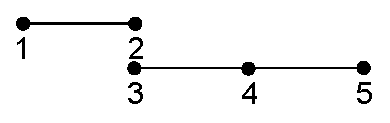
\includegraphics[width=60mm]{Elt1D-ass2.eps}
\end{figure}
La poutre est constituée de la poutre~$1-2$ et de la poutre~$3-4-5$, les points~$2$ et~$3$ étant astreints à rester collés ensembles.
\medskipvm
En ajoutant la relation~$u_2=u_3$ par l'intermédiaire d'un multiplicateur de Lagrange\index{multiplicateurs de Lagrange}\index[aut]{Lagrange (Joseph Louis, comte de -), 1736-1813, Italien}, c'est-à-dire en ajoutant le terme~$\lambda_1(u_2-u_3$), on obtient le système:
\begin{equation}
\MM*{1&-1&0&0&0&0 \\ -1&1&0&0&0&1 \\ 0&0&1&-1&0&-1\\ 0&0&-1&2&-1&0\\ 0&0&0&-1&1&0 \\ 0&1&-1&0&0&0}
\VV*{u_1\\u_2\\u_3\\u_4\\ u_5\\ \lambda_1}
=
\VV*{0\\0\\0\\F' \\ 0 \\ u_d=0}
\end{equation}
auquel il faut également ajouter la condition aux limites~$u_1$=0.

Si cette condition aux limites est imposée par un multiplicateur de Lagrange~$\lambda_2$, alors finalement, il faut résoudre:
\begin{equation}
\MM*{1&-1&0&0&0&0&-1 \\ -1&1&0&0&0&1&0 \\ 0&0&1&-1&0&-1&0\\ 
0&0&-1&2&-1&0&0\\ 0&0&0&-1&1&0&0 \\ 0&1&-1&0&0&0&0 \\ 1&0&0&0&0&0&0}
\VV*{u_1\\u_2\\u_3\\u_4\\ u_5\\ \lambda_1 \\ \lambda_2}
=
\VV*{0\\0\\0\\F' \\ 0 \\ 0 \\ 0}
\qquad \text{ d'où: } 
\left\{\begin{array}{l} u_1=0 \\ u_2=F' \\ u_3=F' \\ u_4=2F' \\ u_5=3F' \\ \lambda_1 = -F' \\ \lambda_2 = -F' \end{array}\right.
\end{equation}
